

\section{Co-creativity, agency and involment}

- So a first question we may ask, related to the core research question, is how this shifting of roles affects human agency
- And how this related to interaction design

- What does creative agency mean?
- To discuss this, let's imagine a spectrum of agency, inspired by Deterding spectrum of creativity
- On one end, we have a human using a computer as a tool. In this case, the agency primary resides in the human
- On the other end, we have a computer autonomously producing, such as experiments like AARON \cite{Cohen1995-wt} or The Painting Fool \cite{Colton2012-jc} and other examples discussed. 
- In the middle, as Deterding proposes \cite{Deterding2017-wh}, we have human-AI co-creativity, where agency is blended. 
- In this case attribution does not belong to one or the other 
- Indeed, agency is central to discussions of co-creativity
- Co-creativity is often described as a blending of agencies, blending of creativity \cite{Moruzzi2024-cq, Lawton2023-tb, Kantosalo2021-mp, Bown2020-oc, Deterding2017-wh, McCormack2020-ix, Bown2015-ig, Moruzzi2022-gp, Inie2023-ml, Palani2024-on, Li2024-yh}
- And I defined it in those terms

\begin{figure}
    \centering
    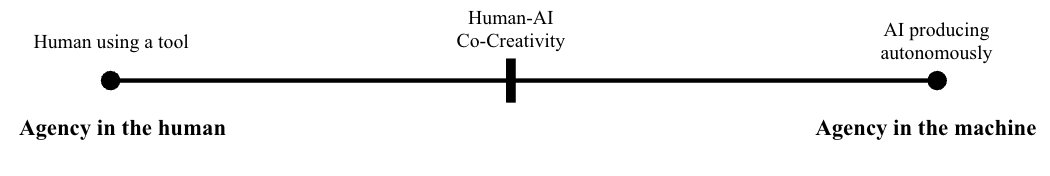
\includegraphics[width=1\linewidth]{agency spectrum.png}
    \caption{Spectrum of agency}
    \label{fig:enter-label}
\end{figure}

- So we may ask the question: where does a human promoting a text to image model sit along that spectrum?
- One may argue it is closer to the AI, since it is mostly an automated production of an image
- The US Patent office explicitely agrees with this view, exemplified when denying copyright to Jason Allen, creator of Opera Spatiale, winner of a digital art competition. Arguing it did not have sufficient human involvement. 

- On the other hand, one could also argue the agency resides in the person. Especially if they iterates multiple times on a prompt. This view also aligns with court ruling related to malicious generating of deep fakes
- Numeros examples exist of people being convicted for the generation of deep fakes. 

- How can we make sense of this dichotomy? 

- I propose the model of intentional and action spaces serves as a useful conceptualisation to resolve it

\section{Defining agency}

- Let's go back to the definition of agency

- Acknowledging it is a highly debated term
I stick here to the what is considered the standard definition of agency as intentional action. \cite{Schlosser2019-jk}

- This introduces a double constraint
- Intention, and the capacity for action 

- A person with intention to act in a certain way but no capacity to do so, has limited agency. 

- Similarly, a person who acts in a certain way, but has no intention to do so, has no agency. 

- Therefore, agency requires the alignment of intention and action. 

- Creative agency requires moving between intention and action spaces 

- A person with agency can move between intention and action spaces gracefully
- In the case of creativity, can move from intention, goals, vision, preferences, towards turning it into outputs.

\section{Severed agency}

- With this, let’s go back to the image prompting question? 

- Where does the agency reside? 

- We can see that it is distributed. 

The human is in the intentional space, providing a prompt which is a intention of an image. 

- The AI exists in the action space, materialising that intention into pixels. 

- Systems that enforce this roles, face the risk of diminishing user agency through a process I term severed agency: the separation between intention and action spaces. 

This happens for three reasons. 

- First: as we have shown, in the literature is clear that adopting this roles and completely separating from the action space leads to skill loss, cognitive skills loss, creative skills loss and worse performance. This ultimately reduces agency and the ability to intentionally create things.

- In contrast, in systems where human is closely involves not only providing instructions but also contributing at the artefact level, better performance is achieved. 

Contrast this with a process of a person using a tool. The action spaces are intentional are very closely aligned. If they are drawing, they are also thinking about where to go, in an iterative feedback loop between intention and action. Exercising skills. Ultimately improving them and enhancing the capacity for creative action: growing their creative agency as a result. 



- In a creative collaboration, between musicians, for example. They engage in exchange ideas and visions at the intentional level, and exchange and contribute at the action level \cite{Bown2020-zn}

- In succesful co-creation, each peson mutually growing each others agency for creation, evolving both intention and action spaces, developing new goals an dperspectives, and ways of collaboratively turning them into outputs.